\documentclass[../main.tex]{subfiles}
\begin{document}


\section{Diseño e implementación}
En este apéndice se describen los aspectos técnicos relacionados con el diseño del sistema desarrollado y su implementación práctica. En primer lugar, se justifica la arquitectura software elegida, detallando su estructura modular y los principios que la sustentan. A continuación, se presenta el entorno de desarrollo y ejecución utilizado para implementar el código y entrenar los modelos de segmentación.

Seguidamente, se analiza la organización del proyecto a nivel de directorios y módulos, explicando la función de cada uno dentro del flujo general. Posteriormente, se profundiza en la implementación, tanto del sistema de configuración de experimentos como de los modelos utilizados. Esta sección incluye la definición formal de los experimentos mediante archivos JSON, su validación mediante Pydantic, y la relación entre las clases mediante un diagrama UML.

Finalmente, se detallan las implementaciones específicas de los modelos empleados: FSRCNN para super-resolución, U-Net para segmentación semántica y YOLO para segmentación basada en polígonos. Se concluye con una sección dedicada a los hiperparámetros utilizados durante el entrenamiento de los modelos, y una tabla comparativa entre ambas arquitecturas.


\subsection{Arquitectura software}
La estructura del proyecto se ha diseñado siguiendo un enfoque modular, con el objetivo de facilitar su implementación, mantenimiento, escalabilidad y reutilización a lo largo del tiempo. Cada componente del sistema —desde el preprocesamiento de imágenes hasta la evaluación de los resultados— está encapsulado en módulos independientes, con responsabilidades claramente definidas. Esta separación lógica no solo favorece una organización más limpia y comprensible del código, sino que también permite desarrollar, probar y modificar cada parte del sistema de forma aislada, minimizando el riesgo de errores colaterales al introducir cambios.

Una de las principales ventajas de este enfoque es la ejecución desacoplada de los módulos. Por ejemplo, es posible ejecutar únicamente el preprocesamiento de las imágenes y almacenar los resultados intermedios para su uso posterior en la fase de entrenamiento, sin necesidad de repetir todo el flujo. De igual modo, se puede cambiar el modelo de segmentación (por ejemplo, de U-Net a YOLO) sin alterar el resto de etapas, lo que favorece la experimentación con distintas arquitecturas y técnicas de forma eficiente.

Además, esta estructura modular permite ejecutar tareas en paralelo o distribuir la carga de trabajo si se dispone de los recursos necesarios. Por ejemplo, se puede realizar el preprocesamiento de nuevas imágenes mientras se entrena un modelo previamente configurado, lo cual mejora significativamente el aprovechamiento del tiempo y de los recursos computacionales disponibles. Esta capacidad de paralelización sería mucho más difícil de implementar en un sistema monolítico, en el que las distintas fases del proceso estarían fuertemente acopladas y dependientes entre sí.

Desde el punto de vista del mantenimiento, el diseño modular también permite detectar y aislar errores de forma más eficiente, así como incorporar nuevas funcionalidades sin necesidad de reescribir grandes partes del código existente. Por ejemplo, se podrían incluir fácilmente nuevas técnicas de preprocesamiento, arquitecturas de red o métricas de evaluación simplemente añadiendo nuevos módulos o extendiendo los existentes.

En cuanto a la escalabilidad, este sistema es también ventajoso. Si se desea introducir, por ejemplo, una nueva red o ampliar el preprocesado o añadir nuevas métricas, solo hay que modificar el módulo correspondiente y si es preciso las conexiones con el resto de módulos.

En resumen, el uso de una arquitectura modular ha sido clave para dotar al sistema de flexibilidad, claridad y capacidad de adaptación, aspectos fundamentales en un proyecto experimental como este, donde la comparación de diferentes enfoques y configuraciones es una parte esencial del trabajo.


\begin{figure}
    \centering
    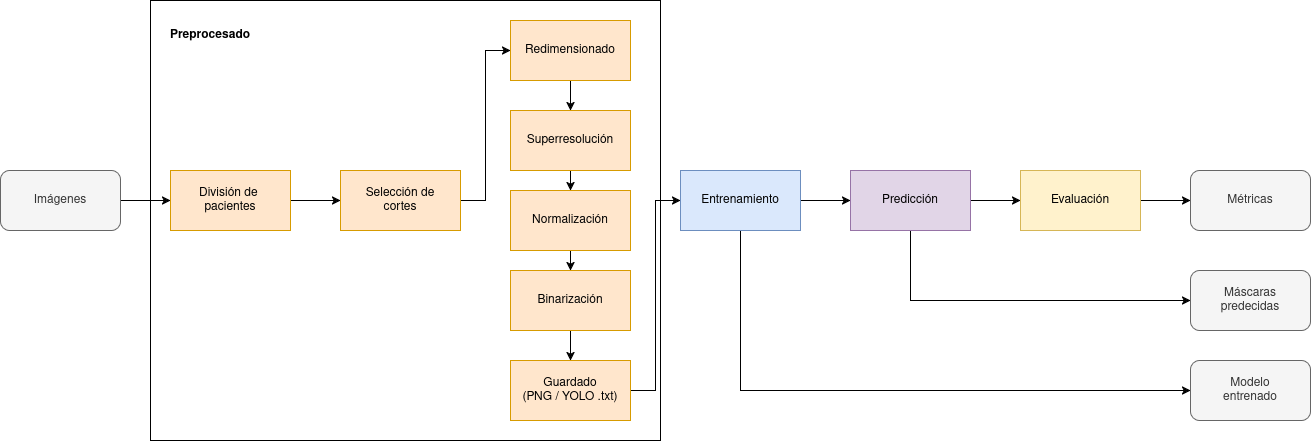
\includegraphics[width=1\textwidth]{imgs/impl/flujo-pipeline.drawio.png}
    \caption{Diagrama del sistema implementado.}
    \label{fig:pipeline-1}
\end{figure}

La Figura \ref{fig:pipeline-1} ilustra el flujo general del sistema a alto nivel. El proceso comienza con la lectura de las imágenes de entrada, que posteriormente se someten a una fase de preprocesamiento, procesando las transformaciones de forma secuencial. A continuación, los datos procesados se utilizan en las etapas de entrenamiento, predicción y evaluación. Estas tres etapas genera tres tipos de salida respectivamente: el modelo entrenado (en formato \texttt{.pth} para U-Net y \texttt{.pt} para YOLO), las métricas de rendimiento calculadas (almacenadas en formato JSON) y las máscaras de segmentación predichas (guardadas como archivos PNG).

\subsection{Entorno de desarrollo}

El desarrollo del proyecto se ha llevado a cabo en dos entornos principales, ambos con sistema operativo Linux: un equipo personal y la plataforma Google Cloud, utilizada para el entrenamiento de modelos en GPU.

\begin{itemize}
    \item \textbf{Equipo local}: portátil con procesador Intel Core i9-13900H de 13ª generación, 32~GB de RAM y tarjeta gráfica NVIDIA RTX 4060 con 8~GB de memoria dedicada. Este entorno se utilizó tanto para la implementación del código como para la validación y pruebas preliminares.
    
    \item \textbf{Equipo remoto}: se utilizó una máquina remota para los entrenamientos de los modelos conectándo a través de SSH, con dos GPUs NVIDIA RTX A6000, cada una con 48~GB de memoria dedicada y una memoria RAM de 128GB.
\end{itemize}

El proyecto está escrito enteramente en \textbf{Python}, gestionado mediante un entorno virtual creado con \textbf{venv}, donde se instalaron todas las dependencias necesarias para garantizar la portabilidad y reproducibilidad de los experimentos. A continuación, se detallan las principales bibliotecas utilizadas:

\begin{itemize}
    \item \texttt{segmentation-models-pytorch}: empleada para implementar la arquitectura U-Net con codificador \texttt{ResNet34}.
    \item \texttt{ultralytics}: utilizada para la integración de modelos YOLO en tareas de segmentación.
    \item \texttt{SimpleITK} y \texttt{nibabel}: para la lectura y manipulación de imágenes médicas en formato NIfTI.
    \item \texttt{scikit-learn}: proporciona las funciones para la validación cruzada.
    \item \texttt{Pillow} y \texttt{matplotlib}: para la visualización y el guardado de resultados.
    \item \texttt{loguru}: para el registro de logs y mensajes de depuración.
    \item \texttt{pydantic}: para la validación de los parámetros necesarios para instanciar las distintas clases.
    \item \texttt{google-cloud-storage}: para guardar los resultados de los modelos en la nube de Google en caso de trabajar con Vertex AI.
\end{itemize}

El control de versiones del proyecto se ha realizado mediante un repositorio privado en GitHub, lo cual ha permitido mantener un historial estructurado del código, facilitar el trabajo modular y garantizar la trazabilidad de los cambios a lo largo del desarrollo del trabajo.


\subsection{Estructura del proyecto}
El programa desarrollado es una herramienta de línea de comandos (\textit{Command Line Interface}, CLI) que requiere un archivo de configuración en formato JSON, donde se define la estructura y los parámetros de los experimentos a ejecutar. Se ha optado por utilizar un archivo JSON para centralizar la configuración, ya que el número de parámetros necesarios haría muy complejo su especificación completa a través de la línea de comandos. A continuación, se describe la organización general de carpetas y archivos del proyecto:

\begin{itemize}
    \item \texttt{main.py}: punto de entrada del programa.

    \item \texttt{cli/}: este módulo tiene las funciones encargadas de parsear los argumentos del programa y el archivo de configuración JSON.

    \item \texttt{config/}: contiene la clase centralizada encargada de cargar y guardar las variables de entorno para funcionalidades opcionales.

    \item \texttt{interfaces/}: el flujo de preprocesado está diseñado para que cada parte implemente funcionalidad común definida en este módulo.
    
    \item \texttt{datasets/}: carpeta dedicada al almacenamiento y organización de los datos de entrada, incluyendo imágenes de resonancia y sus máscaras asociadas.
    
    \item \texttt{logs/}: contiene los archivos de registro generados durante la ejecución del entrenamiento y evaluación, permitiendo el seguimiento de resultados y depuración.
    
    \item \texttt{results/}: almacena las salidas generadas por los distintos modelos, incluyendo segmentaciones predichas, métricas de evaluación y visualizaciones.
    
    \item \texttt{schemas/}: define los esquemas del flujo para asegurar la validez de los parámetros de configuración. Por ejemplo, el archivo \texttt{pipeline\_schemas.py} especifica las clases y estructuras necesarias para la correcta configuración del proceso.
    
    \item \texttt{net/}: contiene las implementaciones de los modelos de red neuronal utilizados:
    \begin{itemize}
        \item \texttt{FSRCNN/}: implementación de la red de super-resolución basada en FSRCNN, incluyendo modelos preentrenados para escalado x2, x3 y x8.
        \item \texttt{unet/}: contiene la implementación de la arquitectura U-Net empleada para la segmentación de imágenes médicas.
        \item \texttt{yolo/}: incluye la configuración y modelo de YOLO adaptado para la tarea de segmentación, con su archivo de configuración \texttt{yolo\_config.yaml}.
    \end{itemize}
    
    \item \texttt{steps/}: estructura clave del proyecto que organiza el flujo de trabajo completo mediante submódulos claramente diferenciados:
    \begin{itemize}
        \item \texttt{preprocessing/}: implementación de la preparación de los datos, división del conjunto, aplicación de la super-resolución y guardado de imágenes resultantes.
        \item \texttt{training/}: módulo encargado del entrenamiento de los modelos.
        \item \texttt{prediction/}: implementación de la lógica de inferencia y generación de predicciones a partir de los modelos entrenados.
        \item \texttt{evaluation/}: scripts para la evaluación cuantitativa y cualitativa de los resultados.
    \end{itemize}
\end{itemize}

% hablar aqui del codigo, quiza incluyendo diagramas de clases
\subsection{Implementación del sistema}
A alto nivel, el programa tiene dos componentes: el experimento y el código que lo ejecuta. Los experimentos se definen de forma completamente declarativa a través de archivos en formato JSON. Cada uno de estos archivos representa un experimento individual e incluye los pasos del flujo a ejecutar (preprocesamiento, entrenamiento, predicción y evaluación), junto con los parámetros específicos requeridos por cada módulo. Estos archivos son parseados al inicio del proceso y transformados en instancias de clases de configuración definidas en el módulo \texttt{schemas/pipeline\_schemas.py}. Gracias al uso de la librería Pydantic, estas configuraciones son validadas y tipadas.

\begin{lstlisting}[language=json, caption={Plantilla de archivo de configuración JSON.}]
{
    "id": "<experimento_id>",
    "preprocess": {
        "net": "<'unet' o 'yolo'>",
        "src_path": "<ruta a al dataset>",
        "dst_path": "<ruta donde escribir los resultados>",
        "resize": [320, 320],
        "split": 0.7,
        "seed": 42,
        "strategy": "<'all_slices', 'lesion_slices', 'brain_slices'>",
        "super_scale": <1, 2, 3, 8>
    },
    "train": {
        "net": "<igual que preprocess.net>",
        "src_path": "<ruta al dataset preprocesado>",
        "dst_path": "<donde escribir el modelo entrenados>",
        "batch_size": 16,
        "use_kfold": false,
        "epochs": 25,
        "learning_rate": 0.001
    },
    "predict": {
        "net": "<igual train.net>",
        "model_path": "<ruta/al/modelo/entrenado>",
        "src_path": "<ruta a las mascaras>",
        "dst_path": "<ruta donde escribir las predicciones>"
    },
    "evaluate": {
        "net": "<igual que train.net>",
        "model_path": "<ruta/al/modelo/entrenado>",
        "src_path": "<ruta al dataset resultado del paso predict>",
        "pred_path": "<ruta donde guardar metricas>",
        "gt_path": "<directorio donde estan las mascaras ground-truth>"
    }
}
\end{lstlisting}

Por otra parte está el código que ejecuta el experimento. Este código se organiza en clases, véase la Figura~\ref{fig:clases}. Todas las clases de configuración heredan de \texttt{BaseModel} (Pydantic), lo que permite la validación automática y la gestión estructurada de los parámetros definidos en archivos JSON. La clase central, \texttt{PipelineConfig}, encapsula de forma opcional una de las configuraciones posibles del sistema: \texttt{PreprocessConfig}, \texttt{TrainConfig}, \texttt{PredictConfig} o \texttt{EvaluateConfig}. Cada una de estas clases define los parámetros específicos necesarios para ejecutar su correspondiente etapa del pipeline. La clase \texttt{TrainConfig} tiene parámetros para activar y configurar la validación cruzada usando Kfolds. Se emplean enumeraciones para restringir valores válidos de atributos como la red utilizada (\texttt{Net}), el método de escalado (\texttt{SuperScale}), la estrategia de selección de cortes (\texttt{Strategy}) o el método de redimensionado (\texttt{ResizeMethod}). Finalmente, la clase \texttt{SegmentationMetrics} encapsula las métricas de evaluación empleadas para valorar el rendimiento de los modelos. Finalmente, la clase \texttt{EnvConfig} se encarga de cargar variables de entorno necesarias para usar funcionalidades opcionales. %como el envío de notificaciones durante el entrenamiento o la subida de los resultados generados por programa a un bucket de Google Cloud. 

\begin{figure}
    \centering
    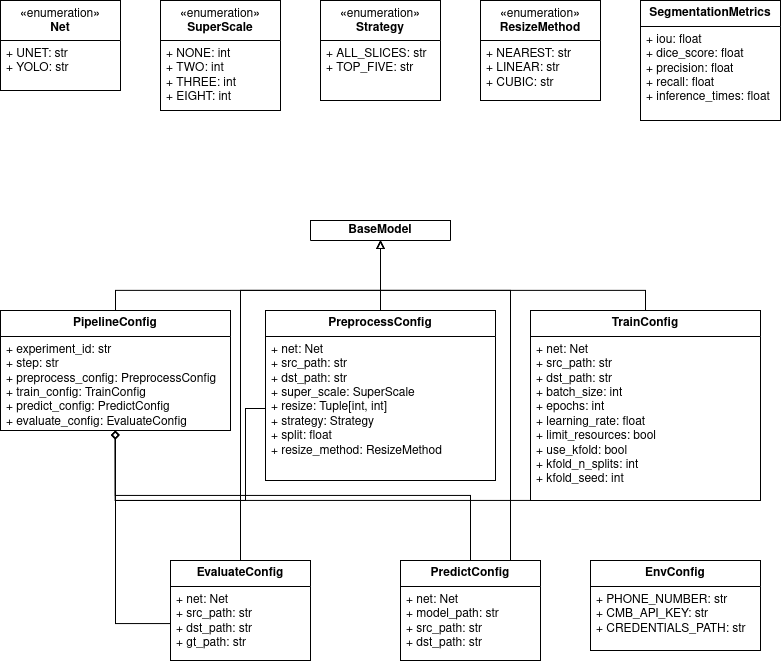
\includegraphics[width=0.8\linewidth]{imgs//impl/diag-clases.drawio.png}
    \caption{Diagrama de clases del sistema de configuración del flujo. Se muestra la relación entre las distintas clases que definen los parámetros de ejecución para cada etapa del procesamiento (preprocesado, entrenamiento, predicción y evaluación), así como las enumeraciones utilizadas para acotar los valores válidos. Todas las clases heredan de \texttt{BaseModel} para beneficiarse de la validación automática de Pydantic. La clase \texttt{PipelineConfig} actúa como contenedor central y se relaciona opcionalmente con una única configuración activa.}
    \label{fig:clases}
\end{figure}


Dentro del módulo de preprocesamiento, se ha optado por un diseño basado en clases abstractas e interfaces que permiten una alta flexibilidad, reutilización y extensibilidad de los distintos componentes del flujo. La idea es facilitar el añadir nuevos pasos de preprocesado implementando la clase abstracta y añadiendo otra opción al archivo de configuración. El módulo se estructura en cuatro componentes principales (obsérvese la Figura~\ref{fig:clases-preprocesamiento}), cada uno definido por una clase abstracta :

\begin{figure}
    \centering
    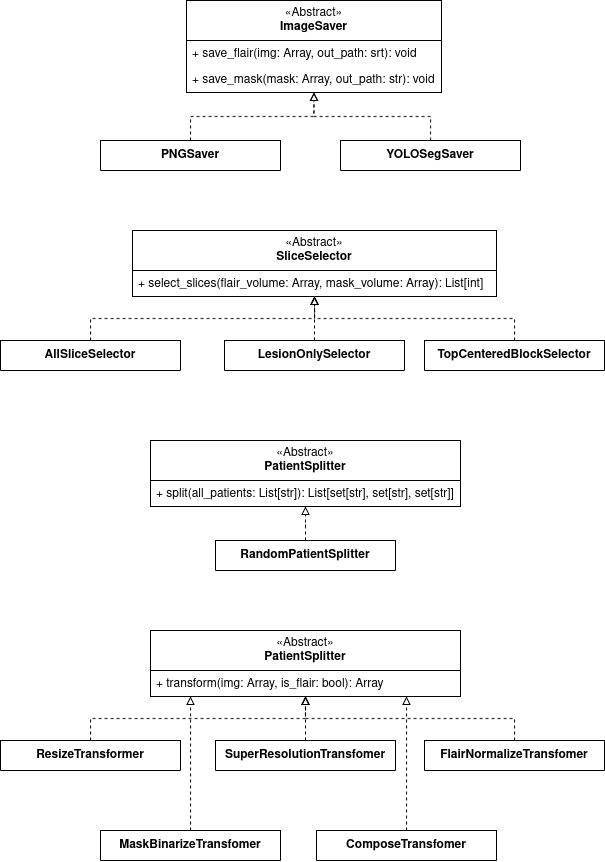
\includegraphics[width=0.8\textwidth]{imgs/impl/preproces-diag-class.drawio.png}
    \caption{Diagrama de clases del sistema de preprocesamiento.}
    \label{fig:clases-preprocesamiento}
\end{figure}



\begin{itemize}
    \item \textbf{ImageSaver}: define la interfaz para guardar imágenes FLAIR y máscaras segmentadas. Cuenta con dos implementaciones: \texttt{PNGSaver}, que guarda los datos en formato PNG, y \texttt{YOLOSegSaver}, que además convierte las máscaras a formato compatible con segmentación en YOLO (polígonos normalizados en archivos \texttt{.txt}).

    \item \textbf{SliceSelector}: abstrae la lógica de selección de cortes 2D a partir de volúmenes 3D. Entre sus implementaciones se encuentran:
    \begin{itemize}
        \item \texttt{AllSliceSelector}: selecciona todos los cortes disponibles.
        \item \texttt{LesionOnlySelector}: selecciona únicamente los cortes con presencia de lesión.
        \item \texttt{BrainSelector}: selecciona los cortes que contienen tejido cerebral, con o sin lesión.
    \end{itemize}

    \item \textbf{PatientSplitter}: define el criterio de división de pacientes entre los subconjuntos de entrenamiento, validación y test.  \texttt{RandomPatientSplitter} realiza esta partición de forma aleatoria pero reproducible, asegurando que no haya solapamiento de pacientes entre subconjuntos.

    \item \textbf{Transformer}: representa una operación de transformación aplicada a una imagen 2D, como redimensionado, normalización o super-resolución. Esta interfaz permite componer múltiples transformaciones mediante la clase abstracta \texttt{ComposeTransformer}. Entre las transformaciones disponibles se incluyen:
    \begin{itemize}
        \item \texttt{ResizeTransformer}: redimensiona la imagen utilizando un método configurable (e.g. \texttt{INTER\_NEAREST} para máscaras).
        \item \texttt{SuperResolutionTransformer}: aplica un modelo FSRCNN únicamente sobre imágenes FLAIR para mejorar su resolución.
        \item \texttt{FlairNormalizeTransformer}: normaliza las intensidades de imágenes FLAIR al rango $[0, 255]$.
        \item \texttt{MaskBinarizeTransformer}: asegura que las máscaras sean estrictamente binarias (valores 0 o 255).
    \end{itemize}
\end{itemize}

Este diseño desacopla completamente la lógica de procesamiento de imágenes del guardado y de la selección de cortes, permitiendo extender o modificar cualquier parte del flujo (por ejemplo, añadir aumentos de datos o nuevos formatos de salida) sin afectar al resto del sistema.


\subsection{FSRCNN}
La implementación utilizada se ha tomado del repositorio  \texttt{FSRCNN-pytorch}\footnote{\url{https://github.com/yjn870/FSRCNN-pytorch}} \cite{fsrcnn_pytorch} y modificada ligeramente. Se proporcionan modelos preentrenados y adaptados para PyTorch. Estos modelos han sido entrenados originalmente con el conjunto clásico de 91 imágenes naturales, conocido como \textit{91-image dataset}, ampliamente utilizado en la literatura para tareas de super-resolución. Para la evaluación del modelo, se emplea también el dataset \textit{Set5}, un conjunto de imágenes de alta resolución usado habitualmente como benchmark. Ambos conjuntos se degradan artificialmente mediante interpolación bicúbica para generar versiones con escalado ×2, ×3 y ×8, que permiten evaluar la capacidad del modelo para reconstruir detalles a partir de imágenes de baja resolución. Esta estrategia permite incorporar super-resolución en el flujo de segmentación sin necesidad de realizar un entrenamiento adicional, reutilizando pesos ya optimizados para mejorar la calidad visual de las imágenes de entrada.

La clase \texttt{FSRCNN} (Figura \ref{fig:fsrcnn-class-diagram}), que hereda de \texttt{torch.nn.Module}, encapsula la arquitectura del modelo. El primer bloque (\texttt{first\_part}) realiza la extracción de características mediante una convolución con kernel 5×5 seguida de una activación PReLU. El segundo bloque (\texttt{mid\_part}) lleva a cabo una compresión dimensional con convoluciones 1×1, seguida de múltiples capas de convoluciones 3×3 y activaciones PReLU que actúan como un mapa de representación interna. Finalmente, el bloque de reconstrucción (\texttt{last\_part}) utiliza una convolución transpuesta con kernel 9×9 para generar una imagen de salida con mayor resolución, escalada por un factor configurable (×2, ×3, ×8).

\begin{figure}
    \centering
    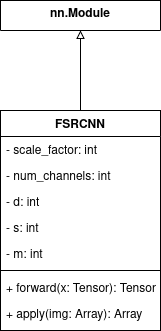
\includegraphics[width=0.25\linewidth]{imgs/impl/fsrcnn-diag-class.drawio.png}
    \caption{Diagrama de clases de la red FSRCNN.}
    \label{fig:fsrcnn-class-diagram}
\end{figure}

Entre sus atributos destacan los parámetros estructurales de la red, como el factor de escalado (\texttt{scale\_factor}), el número de canales de entrada (\texttt{num\_channels}) y los hiperparámetros internos (\texttt{d}, \texttt{s}, \texttt{m}) que controlan el número de filtros y bloques internos de convolución. La clase implementa los siguientes métodos principales:

\begin{itemize}
    \item \texttt{forward(x)}: define el paso hacia adelante del modelo, aplicando las capas secuenciales sobre un tensor de entrada.

    \item \texttt{apply}: aplica super-resolución sobre una imagen de entrada y devuelve la imagen con el nuevo tamaño.
\end{itemize}
    

Esta implementación ha sido adaptada en el módulo \texttt{net/FSRCNN/}, y se compone de tres bloques principales: una capa de extracción de características, un bloque de mapeo no lineal y una etapa de reconstrucción (véase Figura \ref{fig:fsrcnn-impl-arquitectura}).

\begin{figure}[H]
    \centering
    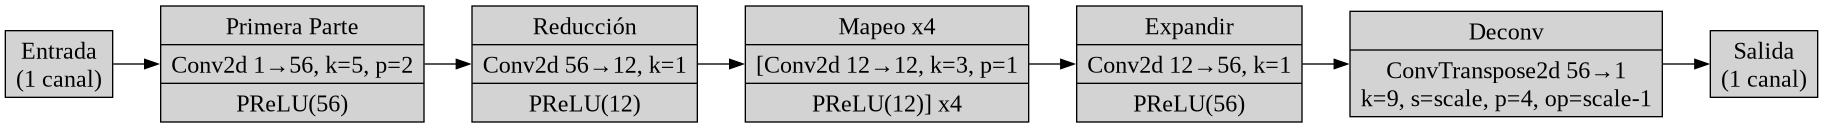
\includegraphics[width=1\linewidth]{imgs/impl/fsrcnn.png}
    \caption{Arquitectura de la red FSRCNN (Fast Super-Resolution Convolutional Neural Network). El modelo toma como entrada una imagen en baja resolución de un solo canal y pasa por una serie de bloques secuenciales: una etapa de expansión inicial (First Part), reducción de canales (Shrink), mapeo no lineal profundo (Mapping), reexpansión de canales (Expand) y una deconvolución final (Deconv) para generar la imagen superresuelta. Cada capa convolucional está seguida por una activación PReLU que mejora la capacidad de aprendizaje del modelo. El parámetro \texttt{scale\_factor} define el grado de super-resolución.}
    \label{fig:fsrcnn-impl-arquitectura}
\end{figure}


\subsection{U-Net}
La implementación de la U-Net tiene un codificador preentrenado ResNet34, adaptada para trabajar con imágenes de resonancia magnética en escala de grises (un canal). Esta elección se fundamenta en la robustez de U-Net para tareas de segmentación médica y en la capacidad de ResNet34 para extraer características profundas de forma eficiente. En La Figura~\ref{fig:unet-class-diag} se muestra el diagrama de clases correspondiente a la implementación de la arquitectura U-Net dentro del sistema desarrollado. Este modelo ha sido encapsulado en una clase principal llamada \texttt{Unet}, la cual centraliza la lógica de entrenamiento, predicción y evaluación del modelo.

\begin{figure}
    \centering
    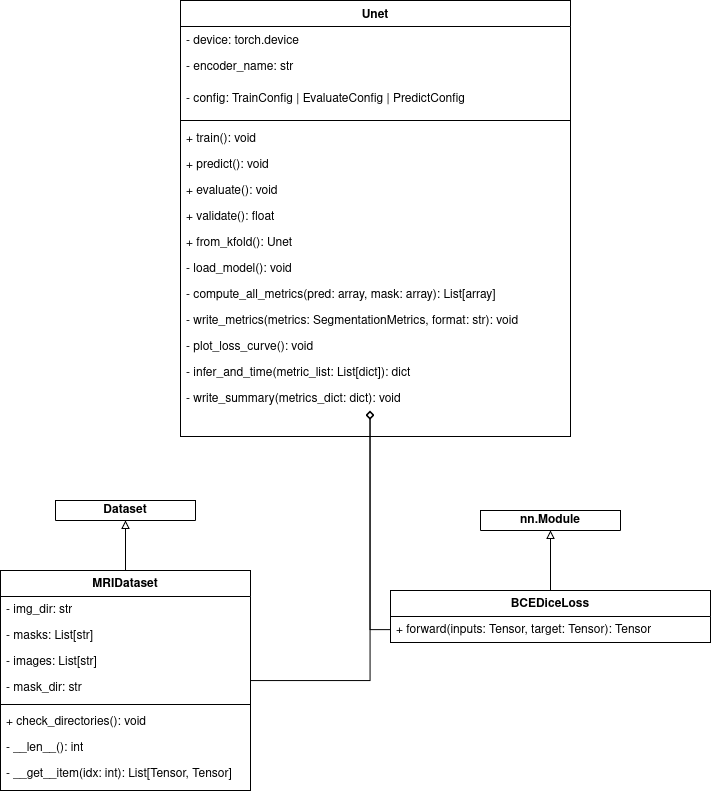
\includegraphics[width=0.65\linewidth]{imgs/impl/unet-class-diag.drawio.png}
    \caption{Diagrama de clases de la red U-Net.}
    \label{fig:unet-class-diag}
\end{figure}

Esta clase contiene los atributos principales necesarios para definir el modelo: el dispositivo de cómputo (\texttt{device}), el nombre del codificador (\texttt{encoder\_name}) y una instancia de configuración (\texttt{config}) que puede ser de tipo \texttt{TrainConfig}, \texttt{EvaluateConfig} o \texttt{PredictConfig}, dependiendo del contexto de ejecución. Entre sus métodos públicos más relevantes se encuentran:

\begin{itemize}
    \item \texttt{train()}, \texttt{predict()} y \texttt{evaluate()}, que ejecutan las etapas principales del flujo de entrenamiento.

    \item \texttt{validate()}, que devuelve una métrica de validación para monitorizar el rendimiento durante el entrenamiento.

    \item \texttt{from\_kfold()}, que permite instanciar el modelo en el contexto de validación cruzada.

    \item \texttt{infer\_and\_time()} y \texttt{write\_summary()}, dedicados al análisis del rendimiento y al registro de resultados.

\end{itemize}
    
Además, la clase implementa métodos privados para la carga del modelo (\texttt{load\_model()}), la evaluación de métricas (\texttt{compute\_all\_metrics()}), el guardado de resultados (\texttt{write\_metrics()}), y la visualización de la curva de pérdida (\texttt{plot\_loss\_curve()}). La clase \texttt{Unet} depende de dos componentes externos clave:

\begin{itemize}
    \item \textbf{\texttt{MRIDataset}}, que hereda de \texttt{Dataset} de PyTorch y se encarga de gestionar el conjunto de datos. Define atributos como el directorio de imágenes, listas de rutas de imágenes y máscaras, y métodos para validar la estructura de carpetas, calcular el tamaño del conjunto (\texttt{\_\_len\_\_}) y acceder a los elementos de forma indexada (\texttt{\_\_getitem\_\_}).

    \item \textbf{\texttt{BCEDiceLoss}}, una clase que hereda de \texttt{nn.Module} y representa una función de pérdida personalizada compuesta por la combinación de \texttt{Binary Cross Entropy} y \texttt{Dice Loss}, diseñada para mejorar la segmentación en contextos con clases desbalanceadas.
\end{itemize}

El flujo de trabajo de la red se inicia con la carga de datos mediante \texttt{DataLoader}, que gestiona tanto las imágenes como sus máscaras correspondientes, organizadas en conjuntos de entrenamiento, validación y prueba. Las imágenes se procesan por una red U-Net con las siguientes características:

\begin{itemize}
    \item Codificador: ResNet34 preentrenado (transfer learning).
    \item Entrada: imágenes de un solo canal.
    \item Salida: mapa de segmentación con activación lineal (sin activación final).
\end{itemize}
    
Durante el entrenamiento, la salida del modelo se evalúa con una función de pérdida combinada \texttt{BCEDiceLoss}, que suma la \texttt{Binary Cross-Entropy} con el \texttt{Dice Loss} suavizado:

\begin{equation}
\mathcal{L}(x, y) = \underbrace{\text{BCEWithLogitsLoss}(x, y)}_{\text{Pérdida de entropía binaria}} + \underbrace{1 - \frac{2 \sum_i \sigma(x_i) y_i + \varepsilon}{\sum_i \sigma(x_i) + \sum_i y_i + \varepsilon}}_{\text{Dice Loss}}
\end{equation}

\begin{itemize}
    \item $x$ es la salida cruda del modelo (logits),
    \item $\sigma(x)$ es la función sigmoide aplicada a $x$,
    \item $y$ es la máscara de verdad (ground truth),
    \item $\epsilon = 10e-5$ es un término de suavizado para evitar divisiones por cero.
\end{itemize}
    
Esto permite balancear regiones lesionadas (menores en tamaño) y no lesionadas (mayores) dentro de la imagen. La optimización se realiza mediante Adam, y el aprendizaje se regula con una política de reducción de tasa de aprendizaje (\texttt{ReduceLROnPlateau}) basada en el valor de pérdida de validación. En la fase de evaluación, se carga el modelo entrenado y se calcula el conjunto de métricas descritas en la sección~Metodología. En la fase de predicción, el modelo produce máscaras binarias aplicando una función sigmoid seguida de un umbral de $0.5$. Estas máscaras se guardan como imágenes binarizadas en formato \texttt{uint8}.

\begin{figure}
    \centering
    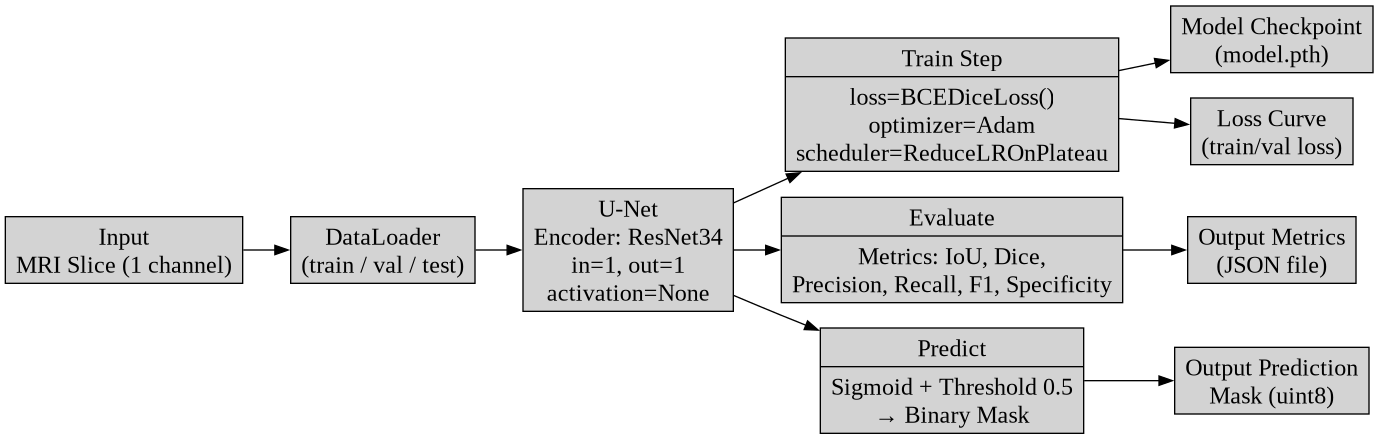
\includegraphics[width=1\linewidth]{imgs/impl/unet.png}
    \caption{Diagrama del sistema de segmentación basado en U-Net.}
    \label{fig:unet-impl-arquitectura}
\end{figure}

En la Figura \ref{fig:unet-impl-arquitectura}, se muestra el flujo de datos desde la entrada de imágenes en escala de grises, el procesamiento mediante la red U-Net con codificador ResNet34, y las tres fases principales: entrenamiento, evaluación y predicción. En el entrenamiento, se emplea la función de pérdida BCEDiceLoss y se genera un modelo entrenado (.pth) junto con curvas de pérdida. En la evaluación, se calculan métricas estándar de segmentación. En la predicción, se exportan máscaras binarias para su análisis posterior.

\subsection{YOLO}
Para la YOLO, se ha utilizado el modelo en su versión de segmentación (\texttt{YOLOv11-seg.pt}), disponible a través de la librería Ultralytics. A diferencia de U-Net y FSRCNN, donde se ha usado la librería \texttt{Torch}, Ultralytics proporciona la implementación de la YOLO junto con todas las herramientas necesarias para trabajar con la red. Por tanto, solo ha sido necesario implementar métodos para: leer y escribir imágenes, calcular y guardar métricas. Además de los tres modos de ejecución: entrenamiento, predicción y evaluación, definidos a través de clases de configuración específicas (TrainConfig, PredictConfig, EvaluateConfig). La Figura~\ref{fig:yolo-class-diag}, representa la clase encargada de encapsular la lógica de entrenamiento, predicción y evaluación la red YOLO.

\begin{figure}
    \centering
    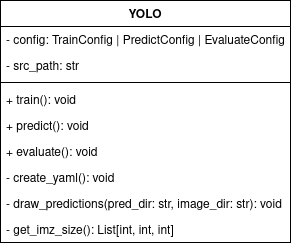
\includegraphics[width=0.5\linewidth]{imgs/impl/yolo-class-diag.drawio.png}
    \caption{Diagrama de clases de la red YOLO.}
    \label{fig:yolo-class-diag}
\end{figure}

Esta clase está diseñada como una interfaz simplificada para interactuar con los modelos provistos por la librería \texttt{ultralytics}. Contiene los siguientes atributos principales:
\begin{itemize}
    \item \texttt{config}: una instancia de \texttt{TrainConfig}, \texttt{PredictConfig} o \texttt{EvaluateConfig}, en función del modo de ejecución.

    \item \texttt{src\_path}: ruta al conjunto de datos de entrada sobre el cual se realiza el entrenamiento, la inferencia o la evaluación. 
\end{itemize}
    
    
Entre sus métodos públicos destacan:
\begin{itemize}
    \item \texttt{train()}, \texttt{predict()} y \texttt{evaluate()}: que implementan las tres etapas fundamentales del ciclo de vida del modelo.

    \item \texttt{create\_yaml()}: encargado de generar automáticamente el archivo de configuración \texttt{data.yaml} requerido por YOLO, en función de las rutas definidas en el experimento y del número de clases.

    \item \texttt{draw\_predictions(pred\_dir, image\_dir)}: que reconstruye las máscaras de segmentación a partir de los archivos de predicción en formato texto (.txt), generando salidas visuales en formato imagen (.png) alineadas con las originales.

    \item  \texttt{get\_imz\_size()}: función auxiliar que devuelve las dimensiones de una muestra del conjunto de datos.
\end{itemize}

En los modos de entrenamiento y predicción, se genera automáticamente un archivo \texttt{data.yaml} (requerido para entrenar el modelo usado) con los siguientes campos:
\begin{itemize}
    \item \texttt{path}: ruta relativa al conjunto de datos.
    \item \texttt{train} y \texttt{val}: rutas internas a imágenes de entrenamiento y validación.
    \item \texttt{nc = 1}: número de clases (solo una clase: “lesion”).
    \item \texttt{names = ["lesion"]}: nombre de la clase.
    \item \texttt{task = "segment"}: tipo de tarea (segmentación semántica).
\end{itemize}

Una peculiaridad de la YOLO es que, a diferencia de las arquitecturas como U-Net, que operan directamente sobre máscaras en formato de imagen (.png), el modelo YOLO en su modalidad de segmentación requiere un formato de entrada diferente: archivos de texto (.txt) que contienen las coordenadas de los polígonos de cada objeto segmentado. Cada archivo de texto describe una imagen del conjunto de entrenamiento o validación y contiene una o más líneas, donde cada línea representa una instancia segmentada mediante un polígono cerrado. La estructura de cada línea es:

\begin{lstlisting}
    <class_id> <x1> <y1> <x2> <y2> ... <xn> <yn>
\end{lstlisting}

\begin{itemize}
    \item \texttt{class\_id} índice entero que representa la clase del objeto (en este caso, siempre 0, ya que solo se segmentan lesiones).
    \item \texttt{x\_i}, \texttt{y\_i}: coordenadas normalizadas (valores entre 0 y 1) de los puntos del contorno del polígono, en orden secuencial.
\end{itemize}

Este formato es obligatorio tanto para entrenamiento como para predicción y está alineado con la filosofía de YOLO de representar objetos como formas geométricas mínimas (cajas, puntos o polígonos) y trabajar sobre texto plano para velocidad y flexibilidad. Dado que el dataset original del proyecto contiene máscaras en formato de imagen binaria (.png), ha sido necesario implementar un paso de preprocesamiento previo que:

\begin{enumerate}
    \item Detecta los contornos de cada máscara.
    \item Extrae los puntos de los polígonos.
    \item Normaliza las coordenadas respecto a la dimensión de la imagen.
    \item Escribe los resultados en archivos .txt compatibles con el formato YOLO segment.
\end{enumerate}
    
Este paso es fundamental para que el modelo pueda ser entrenado correctamente. Del mismo modo, tras la fase de predicción, se implementa una función (\texttt{draw\_predictions}) que:

\begin{enumerate}
    \item Lee los archivos .txt generados por el modelo.
    \item Reconstruye los polígonos a escala original.
    \item Los convierte en máscaras binarias rellenadas para poder evaluar con las métricas.
\end{enumerate}



\end{document}